\documentclass[aspectratio=169]{beamer}
%
% Choose how your presentation looks.
%
% For more themes, color themes and font themes, see:
% http://deic.uab.es/~iblanes/beamer_gallery/index_by_theme.html
%
\mode<presentation>
{
  \usetheme{default}      % or try Darmstadt, Madrid, Warsaw, ...
  \usecolortheme{default} % or try albatross, beaver, crane, ...
  \usefonttheme{default}  % or try serif, structurebold, ...
  \setbeamertemplate{navigation symbols}{}
  \setbeamertemplate{caption}[numbered]
} 

% Set background to black and text to white
\setbeamercolor{background canvas}{bg=black}
\setbeamercolor{normal text}{fg=white}
\setbeamercolor{frametitle}{fg=white}
\setbeamercolor{title}{fg=white}

% You can continue to set other colors as needed:
\setbeamercolor{item}{fg=pink} % Color of bullets
\setbeamercolor{subitem}{fg=yellow}
\setbeamercolor{subsubitem}{fg=cyan}
% ...
\setbeamertemplate{frametitle}[default][center]

\usepackage[english]{babel}
\usepackage[utf8]{inputenc}
\usepackage[T1]{fontenc}
\usepackage{graphicx}

% Set larger font for frame title
\setbeamerfont{frametitle}{size=\huge}

\usepackage{emoji}

\begin{document}

\begin{frame}
    \centering
    \Huge TikTok Successor Proposal \\
    \Huge (Part 1 - Why)
\end{frame}

\begin{frame}{Future Videos}
\begin{columns}[T]
    \begin{column}[T]{0.5\textwidth}
        \begin{itemize}
            \item Part 1: Why replace TikTok?
            \item Part 2: Weird groupchats 
            \item Part 3: Past vertical video
            \item Part 4: Decentralization
            \item Part 5: Redesigned Algorithm
            \item Part 6: Misc / How to help
        \end{itemize}
    \end{column}
    \begin{column}{0.5\textwidth}
        
\includegraphics[height=0.8\textheight]{imgs/app_icons/tiktok-icon2.png}
    \end{column}
\end{columns}
\end{frame}

\begin{frame}{Why Replace TikTok?}
\begin{columns}[T]
    \begin{column}[T]{0.5\textwidth}
        \begin{itemize}
            \item Susceptible to 
            \begin{itemize}
                \item government control 
                \begin{itemize}
                    \item US Ban \emoji{watermelon}
                    \item China 1hr/day limit
                    \item France \& Caledonia??
                \end{itemize}
                \item corporate greed
            \end{itemize}
            \item Need to make nobody in charge
            \begin{itemize}
                \item Solved in Part 4
            \end{itemize}
        \end{itemize}
    \end{column}
    \begin{column}{0.5\textwidth}
        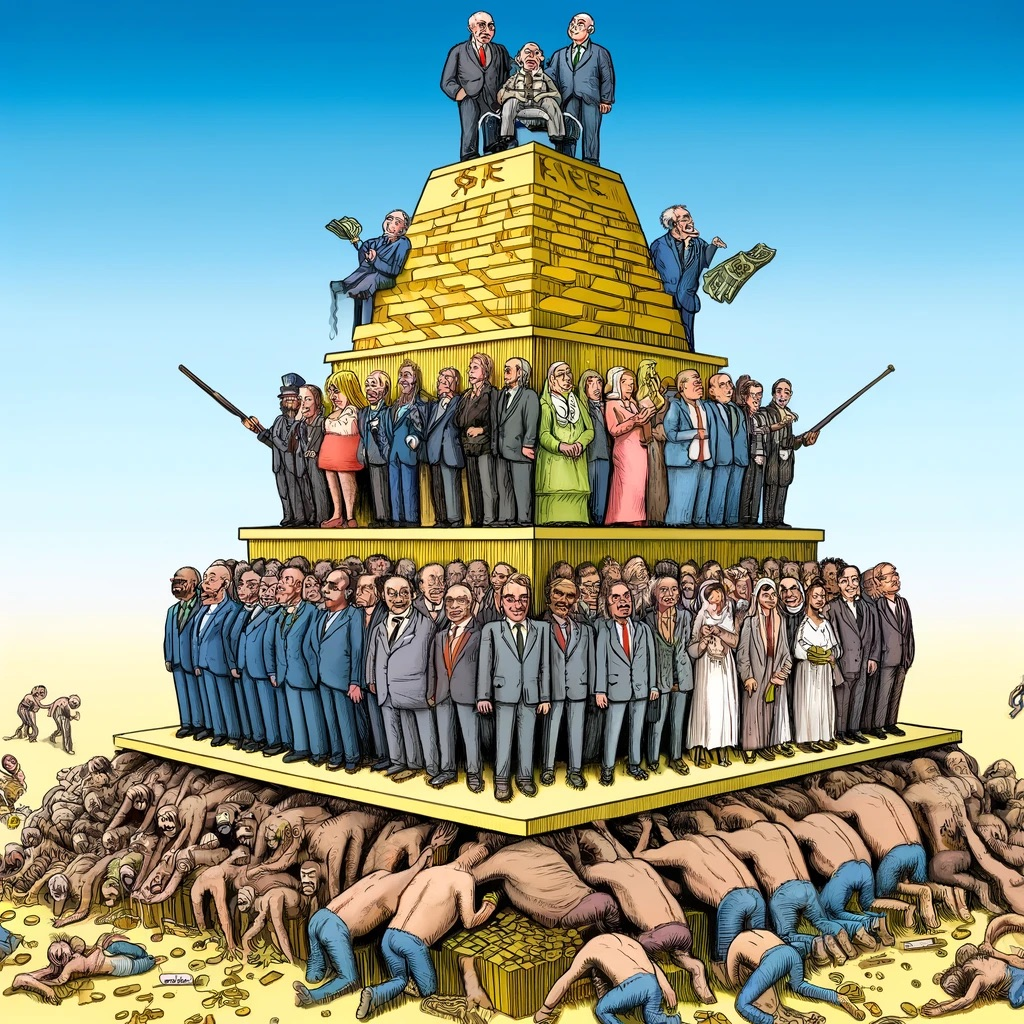
\includegraphics[height=0.8\textheight]{imgs/why_replace/power_pyramid.jpeg}
    \end{column}
\end{columns}
\end{frame}

\begin{frame}{Why Replace TikTok?}
\begin{columns}[T]
    \begin{column}[T]{0.5\textwidth}
        \vspace{0.5in}
        \begin{itemize}
            \item Not the end of history
            \begin{itemize}
                \item Why not try to improve?
            \end{itemize}
        \end{itemize}
    \end{column}
    \begin{column}{0.5\textwidth}
        
\includegraphics[height=0.8\textheight]{imgs/why_replace/future_path.jpeg}
    \end{column}
\end{columns}
\end{frame}

\begin{frame}{Why Replace TikTok?}
\begin{columns}[T]
    \begin{column}[T]{0.5\textwidth}
        \begin{itemize}
            \item Misinformation
            \begin{itemize}
                \item short-form video
                \item difficult to navigate
            \end{itemize}
            \item Need more than just short vertical video
            \begin{itemize}
                \item Solved in Part 3
            \end{itemize}
        \end{itemize}
    \end{column}
    \begin{column}{0.5\textwidth}
        \includegraphics[height=0.8\textheight]{}
    \end{column}
\end{columns}
\end{frame}

\begin{frame}{Why Replace TikTok?}
\begin{columns}[T]
    \begin{column}[T]{0.5\textwidth}
        \begin{itemize}
            \item Echo chamber
            \begin{itemize}
                \item True of all social media
                \begin{itemize}
                    \item Tiktok actually better than most
                \end{itemize}
                \item profit motive $\rightarrow$ want to make you addicted
            \end{itemize}
            \item Need to optionally expose users to diverse viewpoints
            \begin{itemize}
                \item Solved in Part 5
            \end{itemize}
        \end{itemize}
    \end{column}
    \begin{column}{0.5\textwidth}
        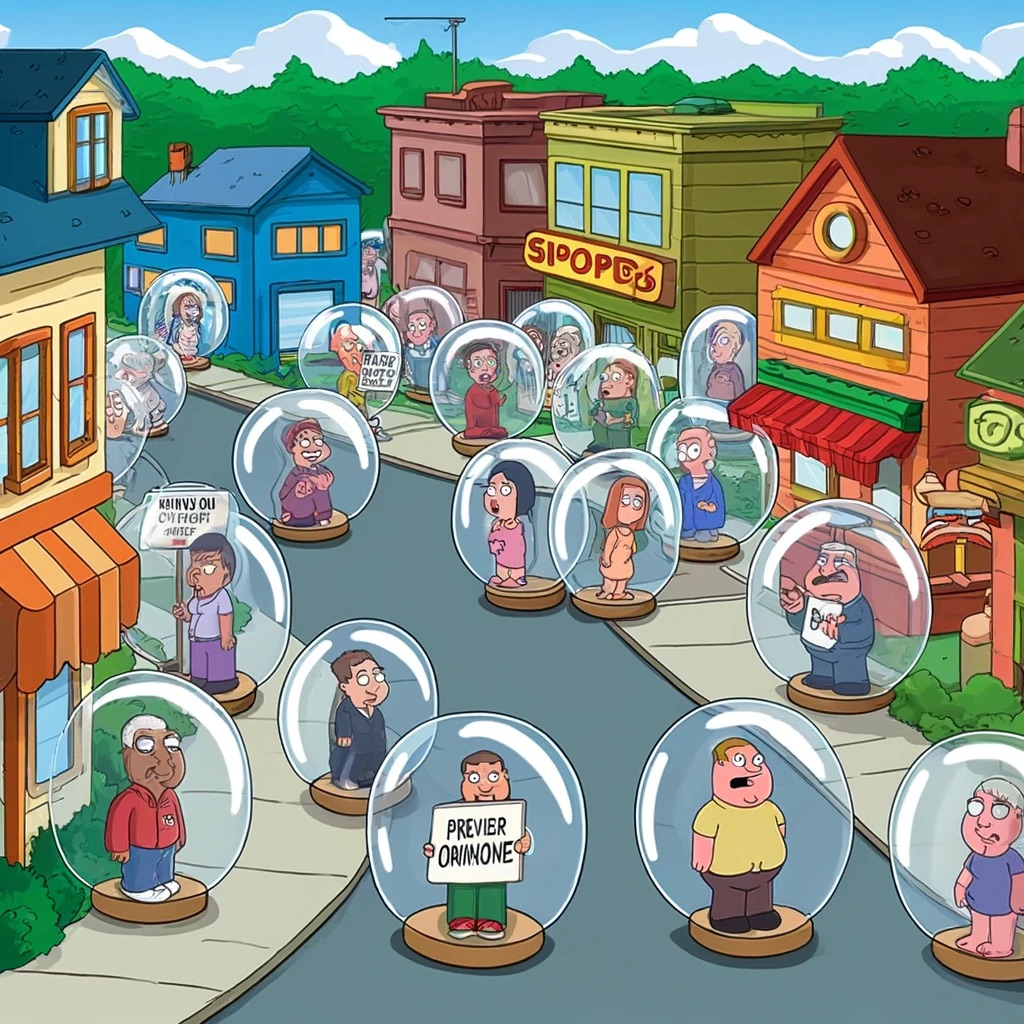
\includegraphics[height=0.8\textheight]{imgs/why_replace/bubble_town.jpeg}
    \end{column}
\end{columns}
\end{frame}

\begin{frame}{Why Replace TikTok?}
\vspace{-0.7in}
\begin{itemize}
    \item Facebook invented online social connection (1-to-1)
    \item Youtube/Instagram created influencers (1-to-all)
    \item Reddit developed shared-interest communities (few-to-few)
    \item Tiktok facilitated global consciousness (all-to-1)/(all-to-few)
    \begin{itemize}
        \item hence \emoji{watermelon} awareness
    \end{itemize}
    \item We need all-to-all, few-to-all, 1-to-few and few-to-1
    \begin{itemize}
        \item Solved in Parts 2 \& 5
    \end{itemize}
\end{itemize}
\end{frame}

\begin{frame}
    \centering
    \Huge TikTok Successor Proposal \\
    \Huge (Part 2 - Groupchats)
\end{frame}

\begin{frame}{Human Communication Has A Problem}
\begin{columns}[T]
    \begin{column}[T]{0.5\textwidth}
        \begin{itemize}
            \item Lots of us \& some louder than others
            \item Can't coordinate without leadership
            \item Good ideas get over-shadowed
            \item Time wasted listening \& filtering instead of deciding \& doing
        \end{itemize}
    \end{column}
    \begin{column}{0.5\textwidth}
        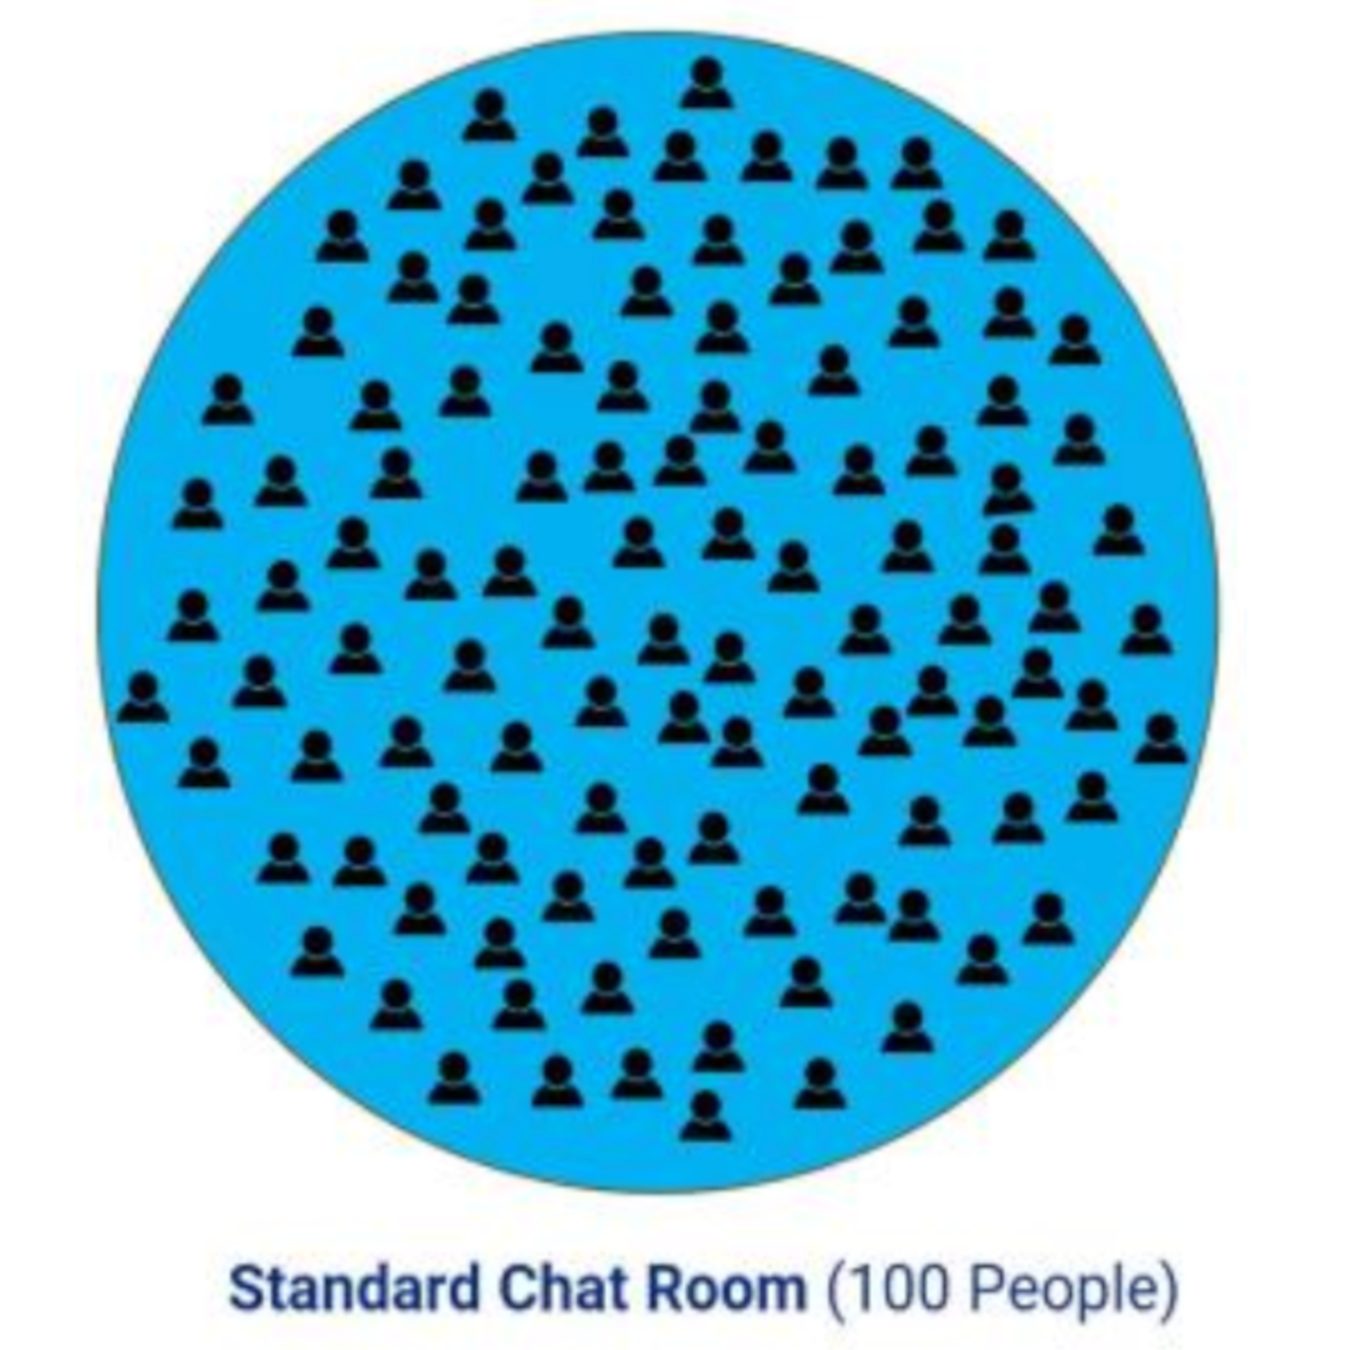
\includegraphics[height=0.8\textheight]{imgs/CSI_section/standard_chat_room.png}
    \end{column}
\end{columns}
\end{frame}

\begin{frame}{Conversational Swarm Intelligence (CSI)}
\begin{columns}[T]
    \begin{column}[T]{0.5\textwidth}
        \begin{itemize}
            \item Break into 20 groupchats of 5 people
            \item ChatGPT periodically summarizes
            \item Other groups receive those summaries
            \item After a few summary exchanges, information that sparks discussion will propogate everywhere
        \end{itemize}
    \end{column}
    \begin{column}{0.5\textwidth}
        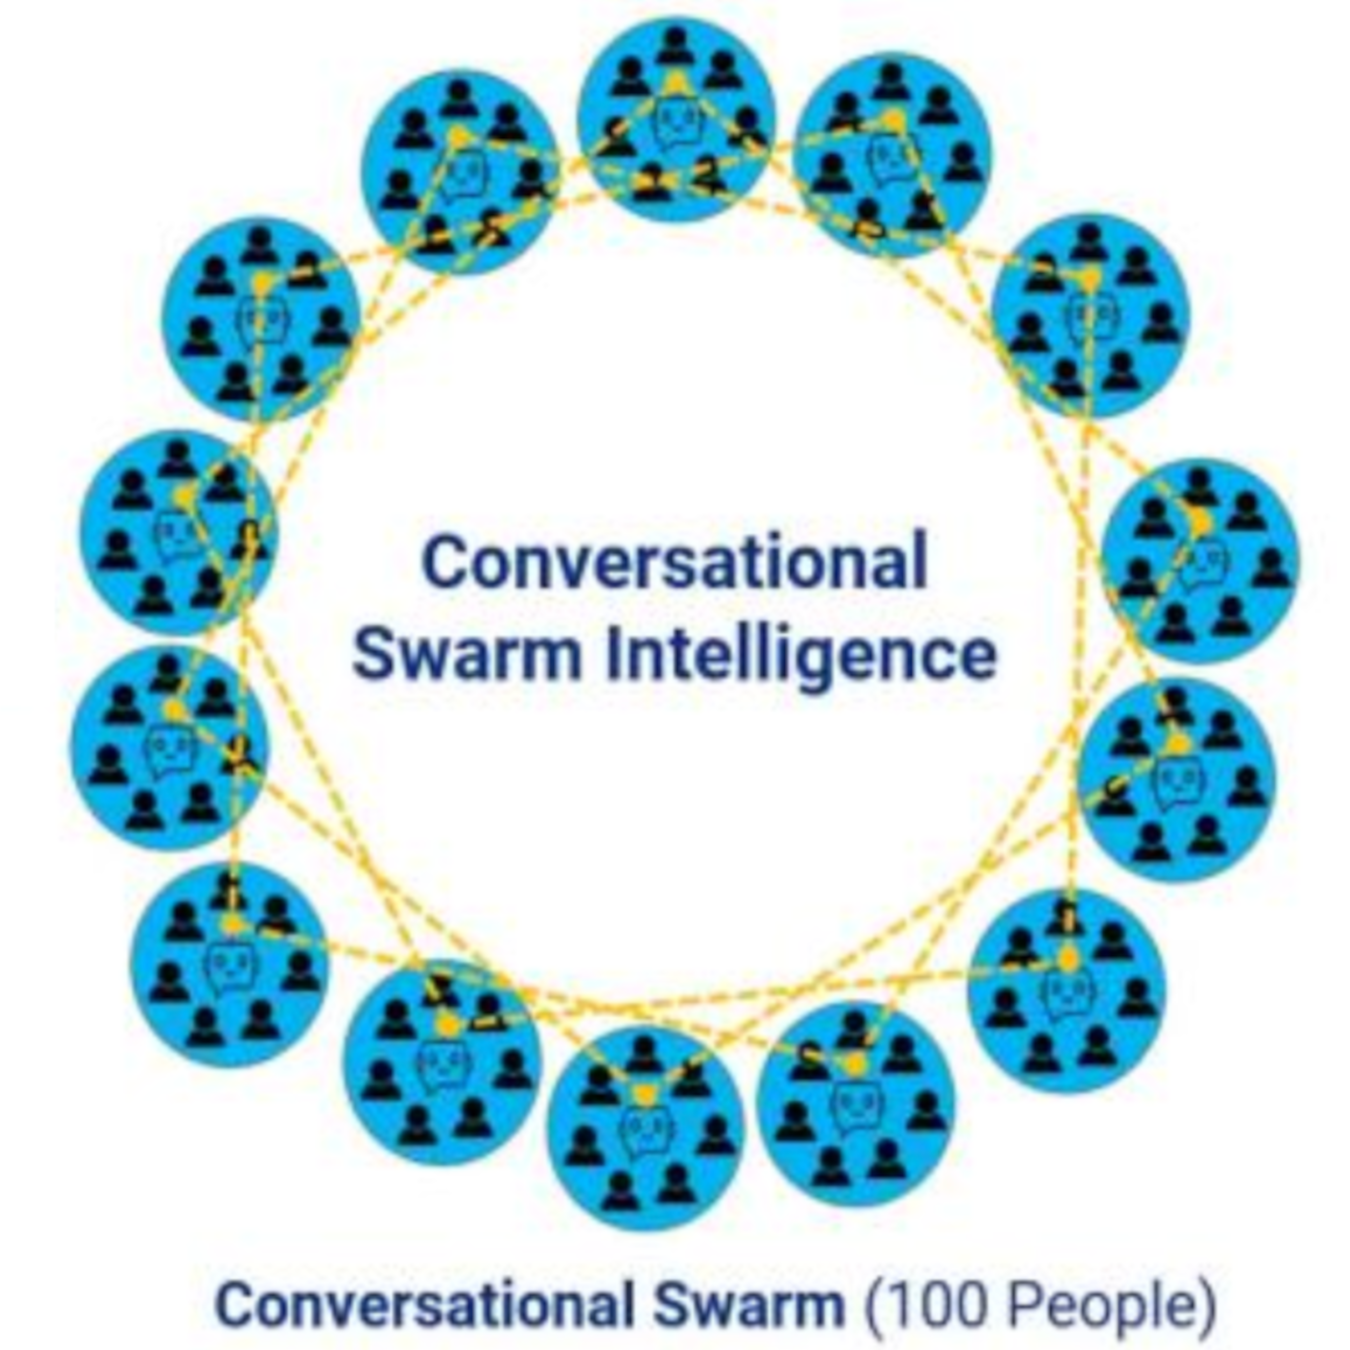
\includegraphics[height=0.8\textheight]{imgs/CSI_section/conversational_swarm.png}
    \end{column}
\end{columns}
\end{frame}

\begin{frame}{Defining a "Summary"}
\begin{columns}[T]
    \begin{column}[T]{0.5\textwidth}
        \begin{itemize}
            \item Learns what you prefer over time
            \item You can directly edit / take over
        \end{itemize}
    \end{column}
    \begin{column}[T]{0.5\textwidth}
        \begin{itemize}
            \item Many settings to fiddle with
            \begin{itemize}
                \item frequency
                \item length
                \item group size
                \item what groups will you join/start?
            \end{itemize}
            \item Customize the content to your group's needs
            \begin{itemize}
                \item meeting minutes (historian)
                \item key takeaways / action items (intern)
                \item criticisms (devil's advocate)
                \item personalize to group that's receiving
            \end{itemize}
        \end{itemize}
    \end{column}
\end{columns}
\end{frame}

\begin{frame}{Hierarchical CSI}
\begin{columns}[T]
    \begin{column}[T]{0.5\textwidth}
        \begin{itemize}
            \item Scales up levels
            \item Groups of ANY size
            \item mix-n-match
        \end{itemize}
    \end{column}
    \begin{column}{0.5\textwidth}
        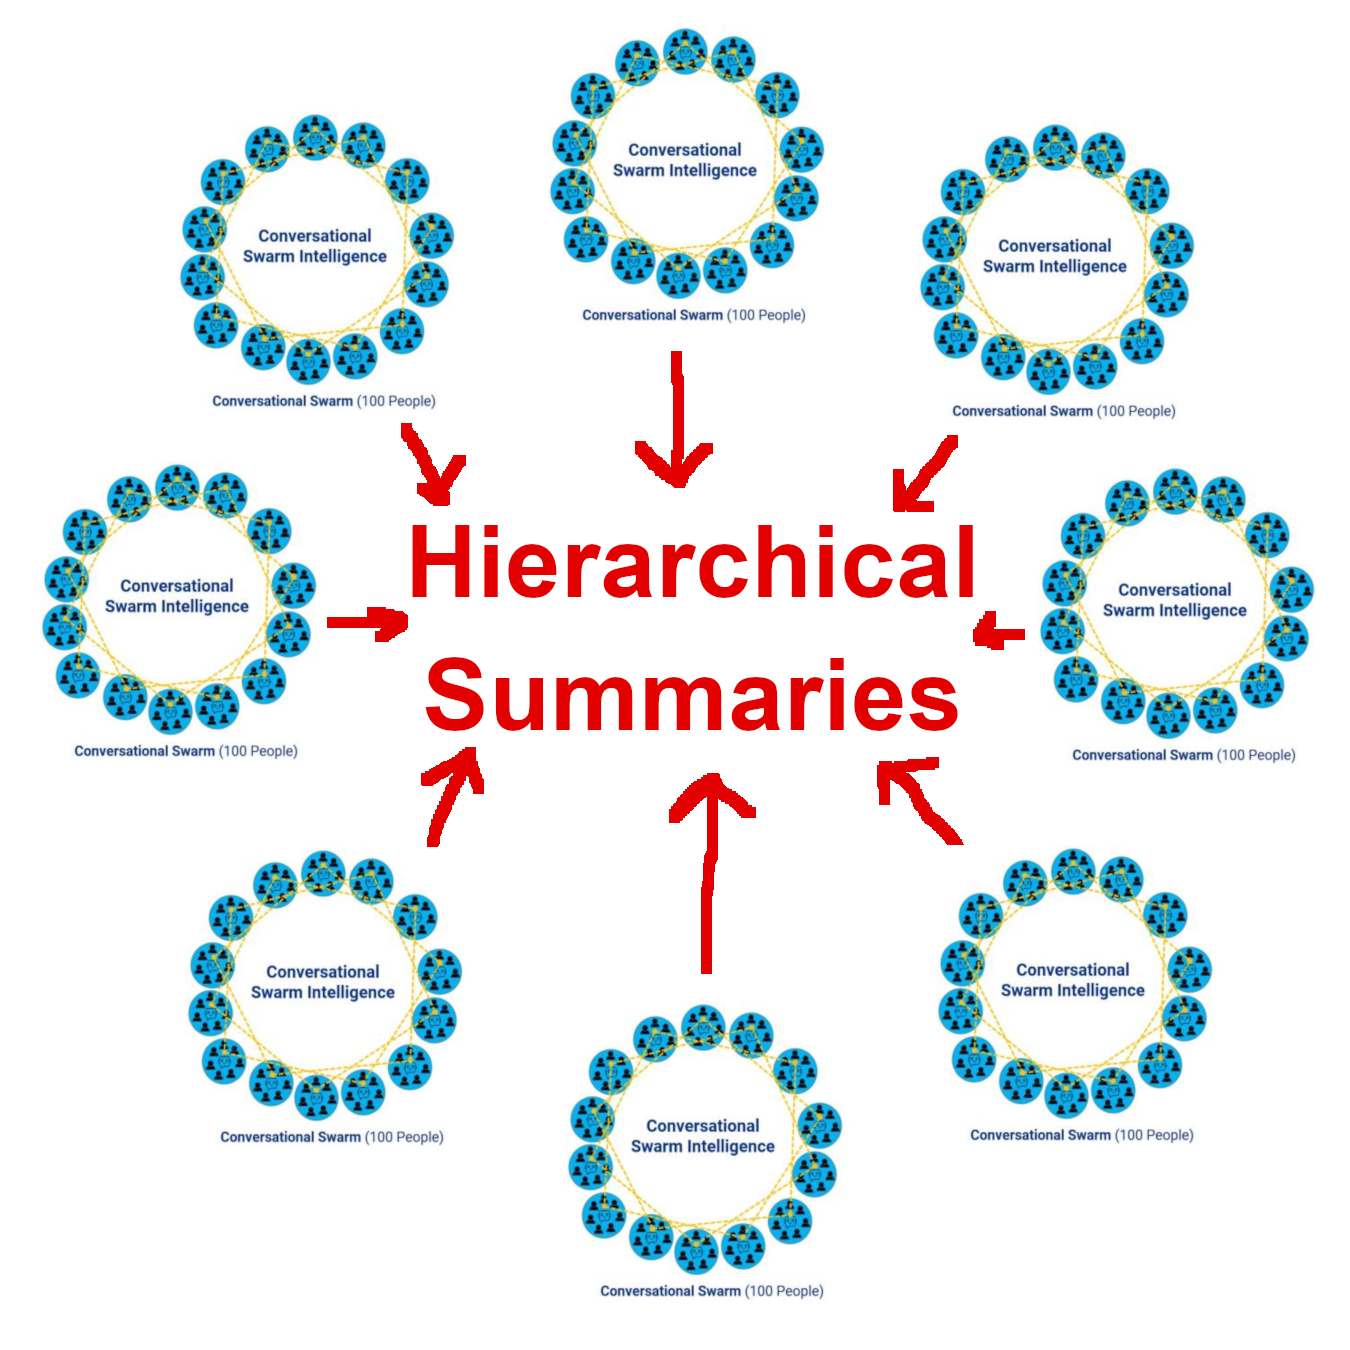
\includegraphics[height=0.8\textheight]{imgs/CSI_section/hierarchical_summaries.png}
    \end{column}
\end{columns}
\end{frame}

\begin{frame}{Interaction w/ World}
\begin{columns}[T]
    \begin{column}[T]{0.5\textwidth}
        \begin{itemize}
            \item talk with an\\ \textit{<insert group name here>}GPT\\ instead of an actual person in that group
            \begin{itemize}
                \item completely optional
            \end{itemize}
            \item talk with groups you otherwise have no exposure/access to
            \item making a public GPT for your group is COMPLETELY OPTIONAL
        \end{itemize}
    \end{column}
    \begin{column}{0.5\textwidth}
        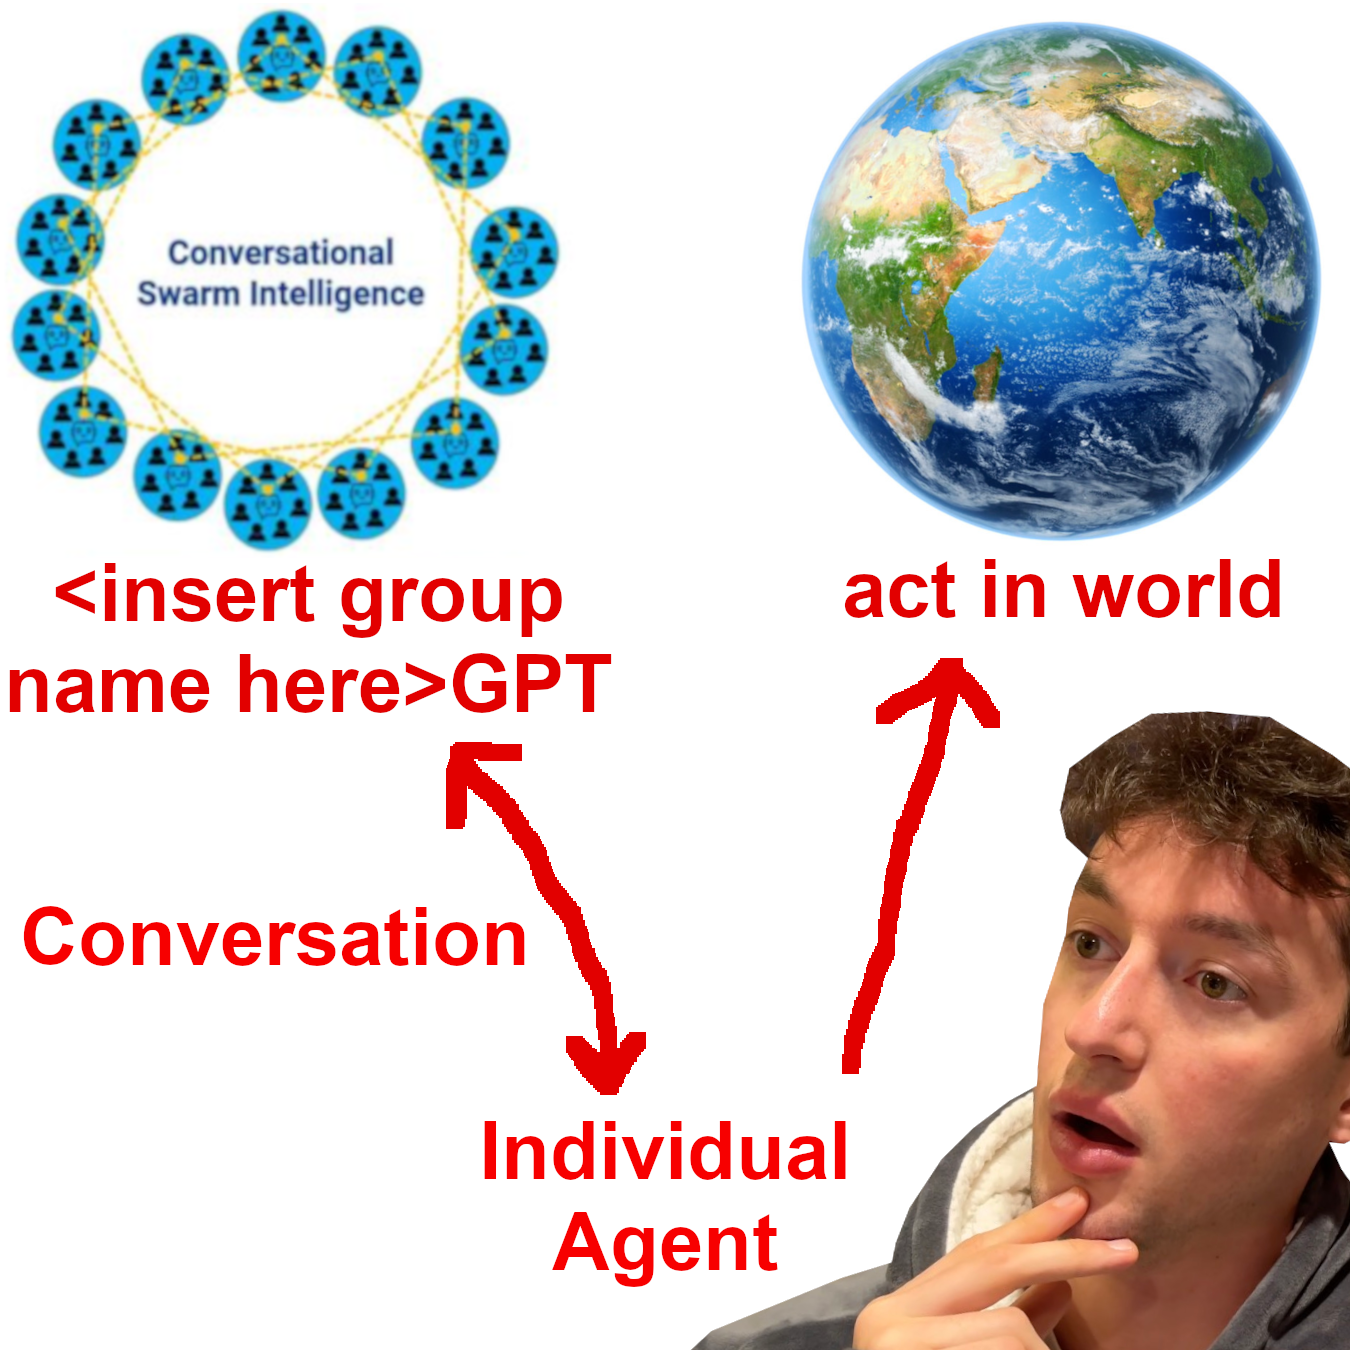
\includegraphics[height=0.8\textheight]{imgs/CSI_section/agency.png}
    \end{column}
\end{columns}
\end{frame}

\begin{frame}{Target Audiences / Use Cases}
\begin{columns}[T]
    \begin{column}[T]{0.5\textwidth}
        \begin{itemize}
            \item Online shared interest communities (Reddit/Discord)
            \item Replace middle-management (Slack)
            \item Grassroots movements won't need leaders or centralized decision making
            \item Local community organization
            \item Literally any large group of people
        \end{itemize}
    \end{column}
    \begin{column}{0.5\textwidth}
        \includegraphics[height=0.8\textheight]{}
    \end{column}
\end{columns}
\end{frame}

\begin{frame}{Credit}
\vspace{-0.5in}
\begin{center}
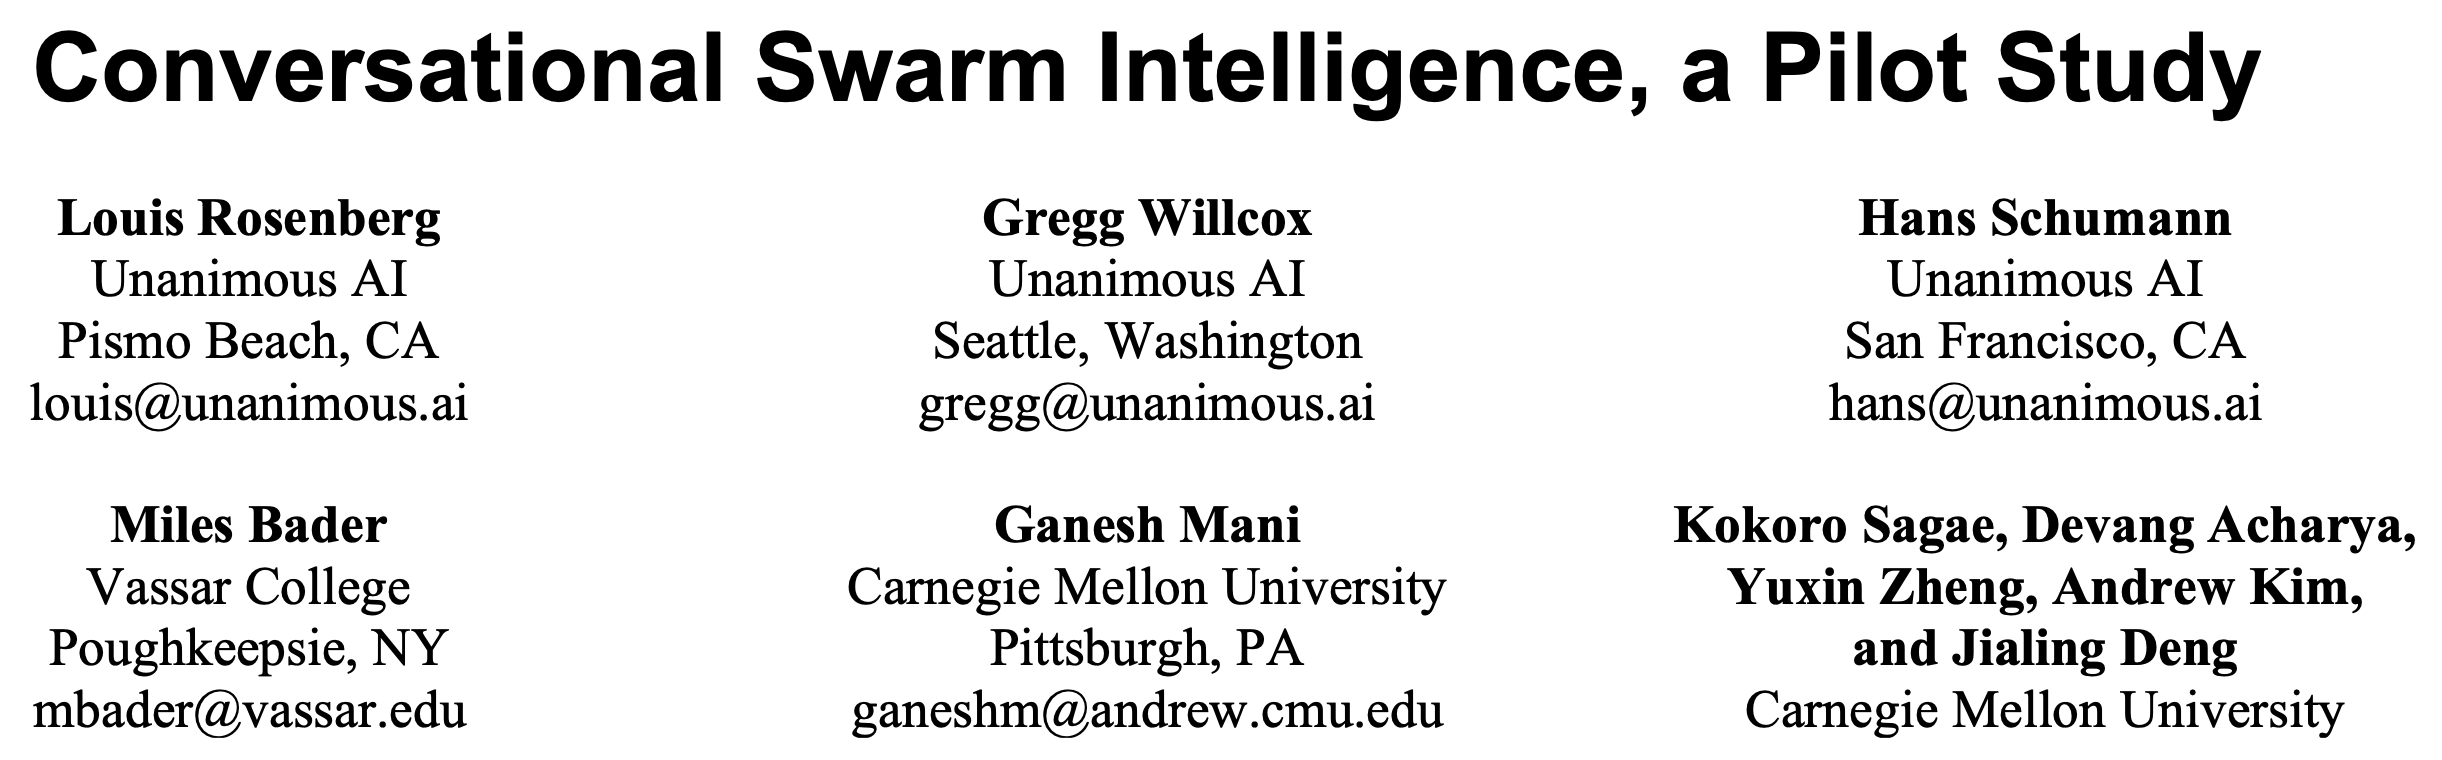
\includegraphics[width=\textwidth]{imgs/CSI_section/authors.png}
\end{center}
\end{frame}

\begin{frame}
    \centering
    \Huge TikTok Successor Proposal \\
    \Huge (Part 3 - Media)
\end{frame}

\begin{frame}{What stays the same}
\begin{columns}[T]
    \begin{column}[T]{0.5\textwidth}
        \begin{itemize}
            \item Short-form vertical video
            \item Algorithm-driven
            \begin{itemize}
                \item More on this in Part 5
            \end{itemize}
        \end{itemize}
    \end{column}
    \begin{column}{0.5\textwidth}
        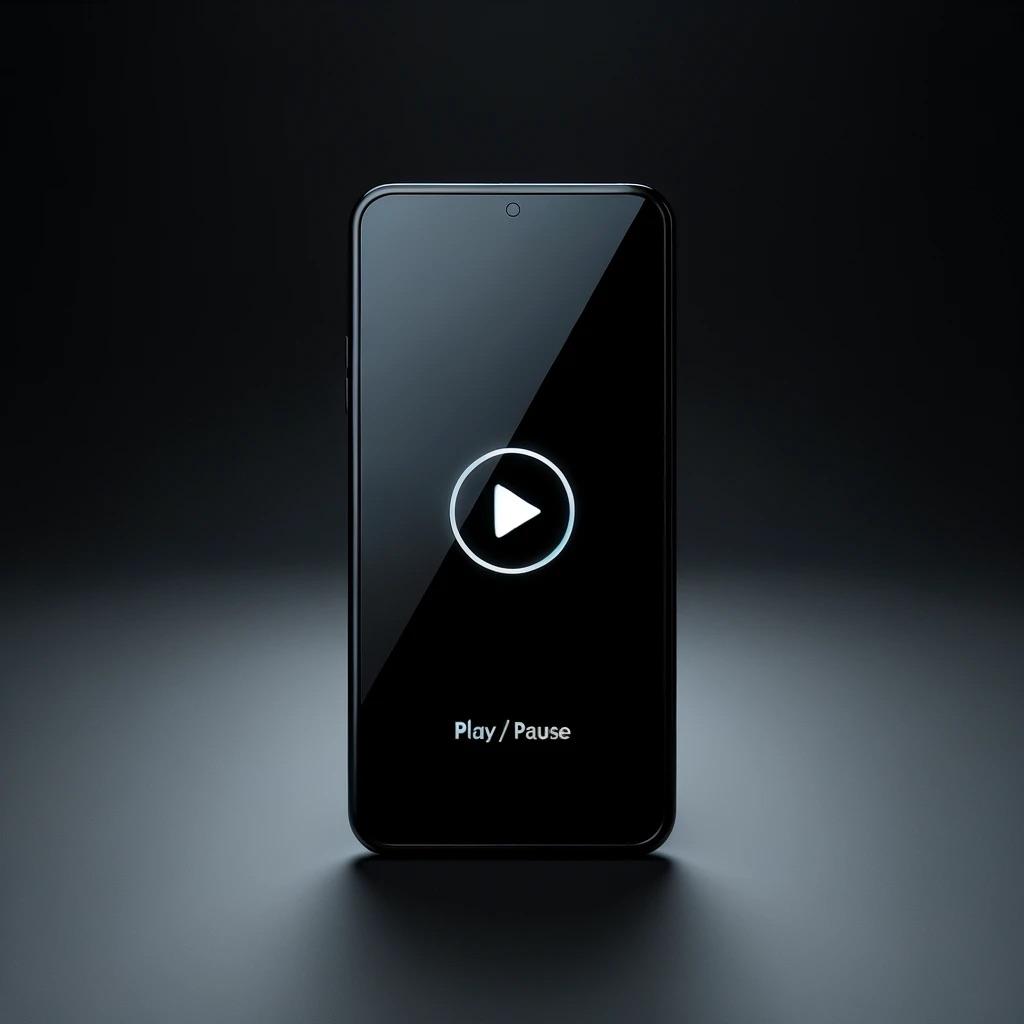
\includegraphics[height=0.8\textheight]{imgs/media/vertical_vid.jpeg}
    \end{column}
\end{columns}
\end{frame}

\begin{frame}{Horizontal Video}
\begin{columns}[T]
    \begin{column}[T]{0.5\textwidth}
        \begin{itemize}
            \item Just rotate your phone
                \item Longer-form content
                \item Introduces whole different part of culture
                \begin{itemize}
                    \item higher detail/quality/rigor
                \end{itemize}
            \item YouTube shouldn't offer me choices
        \end{itemize}
    \end{column}
    \begin{column}{0.5\textwidth}
        
\includegraphics[height=0.8\textheight]{imgs/media/horizontal_vid.jpeg}
    \end{column}
\end{columns}
\end{frame}

\begin{frame}{Written Articles}
\begin{columns}[T]
    \begin{column}[T]{0.5\textwidth}
        \begin{itemize}
            \item Include actual links to sources
            \item Invites "legit" (traditional) journalism
            \item Literally just in your FYP feed
            \item Comment/stitch them to videos
            \item TLDR for me, but Nerds will love
            \item Also tweet-length stuff
        \end{itemize}
    \end{column}
    \begin{column}{0.5\textwidth}
        
\includegraphics[height=0.8\textheight]{imgs/media/quil.png}
    \end{column}
\end{columns}
\end{frame}

\begin{frame}{Conversational Swarm Integration}
\begin{columns}[T]
    \begin{column}[T]{0.5\textwidth}
        \begin{itemize}
            \item Alongside "FYP", "Following", and "STEM" each hive you're a part of will have its own vertical scroll feed
        \end{itemize}
    \end{column}
    \begin{column}{0.5\textwidth}
        \begin{itemize}
            \item In livestreams, the streamer can talk with a swarm summary of the viewers
            \item In groupchats, a ChatGPT can (optionally) be on standby to send videos \& articles relevant to your conversation
            \begin{itemize}
                \item inspiration
                \item fact-checking
                \item counter-arguments
                \item relevant info
            \end{itemize}
        \end{itemize}
    \end{column}
\end{columns}
\end{frame}

\begin{frame}
    \centering
    \Huge TikTok Successor Proposal \\
    \Huge (Part 4 - Decentralization)
\end{frame}

\begin{frame}{Open-Source}
\begin{columns}[T]
    \begin{column}[T]{0.5\textwidth}
        \begin{itemize}
            \item All code is released to the internet, free for anyone to use
            \item Companies, organizations, hobbyists, you, etc can build your own version
            \begin{itemize}
                \item Licensing restrictions on pre-existing companies of a certain size
            \end{itemize}
        \end{itemize}
    \end{column}
    \begin{column}{0.5\textwidth}
        \includegraphics[height=0.8\textheight]{}
    \end{column}
\end{columns}
\end{frame}

\begin{frame}{Modularity/Choice}
\begin{columns}[T]
    \begin{column}[T]{0.5\textwidth}
        \begin{itemize}
            \item EVERYTHING is optional; turn anything off for privacy reasons
            \begin{itemize}
                \item This may result in a reduced experience
            \end{itemize}
            \item Because the code is open-source, you can swap-out our feature for someone else's or your own
        \end{itemize}
    \end{column}
    \begin{column}{0.5\textwidth}
        \includegraphics[height=0.8\textheight]{}
    \end{column}
\end{columns}
\end{frame}

\begin{frame}{Encryption}
\begin{itemize}
    \item Encryption for privacy wherever possible
    \begin{itemize}
        \item Some likely not enabled by default
        \item Likely incompatible with some features, thus restricting quality of experience
    \end{itemize}
    \item Encryption + HCSI competes with Telegram
    \item Even run your own local ChatGPT for HCSI and use it fully encrypted instead of ours
\end{itemize}
\end{frame}

\begin{frame}{Decentralization}
\begin{columns}[T]
    \begin{column}[T]{0.5\textwidth}
        \begin{itemize}
            \item Crypto bros are cringe but... hear me out
            \item Run HCSI entirely on blockchain
            \item AI Recommendation algorithms for your FYP likely require an organization/company/nerd to run
        \end{itemize}
    \end{column}
    \begin{column}{0.5\textwidth}
        \includegraphics[height=0.8\textheight]{}
    \end{column}
\end{columns}
\end{frame}

\begin{frame}
    \centering
    \Huge TikTok Successor Proposal \\
    \Huge (Part 5 - Algorithm)
\end{frame}

\begin{frame}{}
\begin{columns}[T]
    \begin{column}[T]{0.5\textwidth}
        \begin{itemize}
            \item 
        \end{itemize}
    \end{column}
    \begin{column}{0.5\textwidth}
        \includegraphics[height=0.8\textheight]{}
    \end{column}
\end{columns}
\end{frame}

\begin{frame}
    \centering
    \Huge TikTok Successor Proposal \\
    \Huge (Part 6 - Misc / How to Help)
\end{frame}

\begin{frame}{Potential Branding}
\begin{columns}[T]
    \begin{column}[T]{0.5\textwidth}
        \begin{itemize}
            \item Inspiration sources for names (these will make more sense later)
            \begin{itemize}
                \item Intelligent swarm behavior in animals
                \item Bee hives
                \item Spider webs
                \item Chorus, harmonics
                \item Mycelium
            \end{itemize}
        \end{itemize}
    \end{column}
    \begin{column}{0.5\textwidth}
        \begin{tabular}{cc}
            
\includegraphics[width=0.45\textwidth]{imgs/app_icons/1.png} & 
\includegraphics[width=0.45\textwidth]{imgs/app_icons/2.png} \\ 
            
\includegraphics[width=0.45\textwidth]{imgs/app_icons/1.png} & 
\includegraphics[width=0.45\textwidth]{imgs/app_icons/2.png} \\ 
        \end{tabular}
    \end{column}
\end{columns}
\end{frame}


\end{document}
